\justifying
\begin{problem}{1}
	Катет і гіпотенуза прямокутного трикутника дорівнюють відповідно $8$ та $10$ см. Знайдіть
	\begin{multicols}{2}
		\begin{enumerate} 
			\item 
			синус кута, який лежить проти меншого катета
			\item 
			косинус кута, який лежить проти більшого катета
			\item 
			тангенс кута. протилежного до меншого катета
			\item 
			котанегенс кута. прилеглого до меншого катета
		\end{enumerate} 
	\end{multicols}
\end{problem}


\begin{problem}{2}
	Заповніть таблицю
	\begin{table}[h!]
		\centering
		\begin{tabular}{|c|c|c|c|c|c|c|c|c|c|c|}
			\hline
			Градусна міра кута &                   & $12^{\circ}$ & $36^{\circ}$ &                   &                   & $105^{\circ}$ & $225^{\circ}$ &        &          & $240^{\circ}$ \\ \hline
			Радіанна міра кута & $\dfrac{\pi}{18}$ &              &              & $\dfrac{4\pi}{9}$ & $\dfrac{3\pi}{5}$ &               &               & $4\pi$ & $1.8\pi$ &               \\ \hline
		\end{tabular}
	\end{table}
\end{problem}

\begin{problem}{3}
	$\cos \alpha = \frac{1}{3}$. Знайти
	\begin{multicols}{2}
		\begin{enumerate} 
			\item 
			$\tan \alpha$
			\item 
			$\sin \alpha$
			\item 
			$\cot \alpha$
		\end{enumerate} 
	\end{multicols}
\end{problem}

\begin{problem}{4}
	Визначити напрямок та величину суми двох векторів, модулі яких дорівнюють 3 та 4 відповідно, у наступних випадках:
	\begin{enumerate}
		\item
		вектори спрямовані в одному напрямку
		\item
		вектори спрямовані в протилежних напрямках
		\item
		вектори перпендикулярны один одному
		\item
		вектор суми є перпендикулярним до першого вектора
	\end{enumerate}
\end{problem}

\begin{problem}{5}
	Обрати та за допомогою рисунку додати два вектори однакової довжини a так, шоб вектор їх суми за довжиною дорівнював:
	\begin{enumerate}
	\item нулю
	\item був вдвічі більщий за а
	\item мав таку ж саму довжину а
	\item мав довжину в $\sqrt{2}$ разів більшу за а		
	\end{enumerate}

\end{problem}

\begin{figure}[h!]
	\centering
	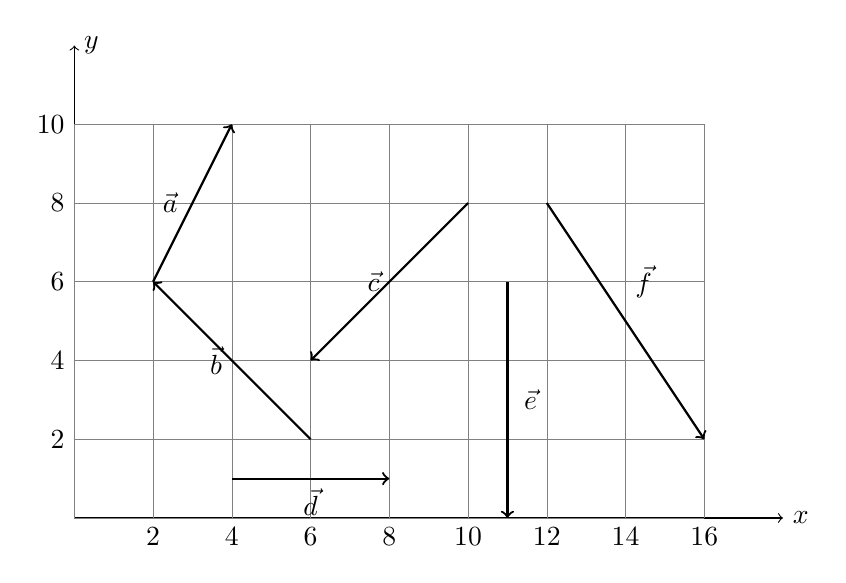
\begin{tikzpicture}<br>
	\draw [->] (0,0) -- (0,6);
	\draw [->] (0,0) -- (9,0);
	\node [right] at (9,0) {$x$};
	\node [right] at (0,6) {$y$};
	\draw[help lines] (0,0) grid (8,5);<br>
	
	\draw [->, thick] (1,3) -- (2,5);
	\node [above, right] at (1, 4) {$\vec{a} $};
	
	\draw [->, thick] (3,1) -- (1,3);
	\node [left] at (2, 2) {$\vec{b} $};
	
	\draw [->, thick] (2,0.5) -- (4,0.5);
	\node [below] at (3, 0.5) {$\vec{d} $};
	
	\draw [->, thick] (5,4) -- (3,2);
	\node [left] at (4, 3) {$\vec{c} $};
	
	\draw [->, thick] (5.5,3) -- (5.5,0);
	\node [left] at (6, 1.5) {$\vec{e} $};
	
	\draw [->, thick] (6,4) -- (8,1);
	\node [right] at (7, 3) {$\vec{f} $};
	
	\node [below] at (1, 0) {$2$};
	\node [below] at (2, 0) {$4$};
	\node [below] at (3, 0) {$6$};
	\node [below] at (4, 0) {$8$};
	\node [below] at (5, 0) {$10$};
	\node [below] at (6, 0) {$12$};
	\node [below] at (7, 0) {$14$};
	\node [below] at (8, 0) {$16$};
	
	\node [left] at (0, 1) {$2$};
	\node [left] at (0, 2) {$4$};
	\node [left] at (0, 3) {$6$};
	\node [left] at (0, 4) {$8$};
	\node [left] at (0, 5) {$10$};
	\end{tikzpicture}
	\caption{до задачі}
	\label{clas_0_vectors}
	
\end{figure}
\begin{problem}{6}
	На рис. \ref{clas_0_vectors} зображене розташування вкторів на координатній площині. Знайти напрямок та величину наступних векторинх виразів. Зобразити графічно:	
 $\vec{c} + \vec{d}, ~\vec{c}+\vec{b}, ~\vec{e}-\vec{f},~ \vec{a}-\vec{c},~ 2\cdot(\vec{b}+\vec{f})$

\end{problem}

\begin{problem}{7}
	Вектори $\vec{a}$ та $\vec{b}$ такі, що $|\vec{a}| = 3,~ |\vec{b}| = 2, ~\angle(\vec{a},\vec{b}) = 60^{\circ}$. Знайдіть
	\begin{enumerate}
		\item |2$\vec{a} + \vec{b}$|
		\item (2$\vec{a}$, $\vec{a}-\vec{b}$)
	\end{enumerate}


\end{problem}

\begin{problem}{16}
	Дано вектори $\vec{a} = (3,1), ~\vec{b} = (1,-2),~\vec{c} = (-1,3)$. За якого значення параметра $k$ вектори $\vec{a}+k\vec{b}$ та $\vec{c}$
	\begin{enumerate}
		\item однаково напрямлені
		\item перпендикулярні
		\item рівні за модулем
	\end{enumerate}
\end{problem}

\textbf{Задачі для самостійного розв'язання}
\begin{problem}{8}
	Траса для велосипедистів має форму прямокутного трикутника, один з кутів якого дорівнює $50^{\circ}$. Меншу сторону цього трикутника один із велосипедистів проїжджає за 1 год. За який час він проїде всю трасу? 
	(швидкість велосиппедиста постійна на всій трасі)
\end{problem}

\begin{problem}{9}
	Доведіть. що площу сектора кола можно знайти за формулою $S = \dfrac{\alpha R^2}{2}$, де $\alpha$ - радіанна міра центрального кута, R - радіус кола
\end{problem}
\begin{problem}{10}
	Знайдіть невідомі сторони прямокутного трикутника ABC ($\angle C = 90^{\circ}$), якщо:
	\begin{enumerate}
		\item $BC = 2 $ см, $\cos B = \dfrac{2}{3}$
		\item $AC = 2 $ см, $\sin B = \dfrac{1}{4}$
	\end{enumerate} 
\end{problem}

\begin{problem}{11}
	Укажіть взаємне розташування ненульових векторів $\vec{a}$ та $\vec{b}$ для яких:
	\begin{enumerate}
		\item $(\vec{a}+\vec{b})\perp (\vec{a}-\vec{b})$
		\item $|\vec{a}+\vec{b}|<|\vec{a}-\vec{b}|$
	\end{enumerate}
\end{problem}

\begin{problem}{12}
	За допомогою скалярного добутку довести теорему Піфагора. (\textit{Вказівка}: представити катети через вектори а гіпотенузу - через суму або різницю векторів)
\end{problem}

\begin{problem}{15}
	Вектор швидкості одного велосипедиста має вигляд $\vec{v}_1 = (9,12)$, другого -- $\vec{v}_2 = (5,12)$. Знайти кут між напрімками руху велосипедистів
\end{problem}

\begin{problem}{13}
	Обчилсити довжини діагоналей та кут між діагоналями паралелограма, побудованого на векторах $\vec{a} = 5\vec{p} + 2\vec{q}, ~\vec{b} = \vec{p}-3\vec{q}$, якщо
	\begin{enumerate}
		\item $|\vec{p}| = 2\sqrt{2}, ~|\vec{q}| = 3, ~\angle(\vec{p},\vec{q}) = 45^{\circ}$
		\item $\vec{p} = (1,2),~ \vec{q} = (3,-1)$
	\end{enumerate}
\end{problem}

\begin{problem}{14}
	Знайдіть розклад вектора $\vec{c}$ за векторами $\vec{a},~\vec{b}$ якщо
	\begin{enumerate}
		\item $\vec{a} = (-1,2),~\vec{b} = (4,3), ~\vec{c} = (5,12)$
		\item $\vec{a} = (2,-3),~\vec{b} = (1,2), ~\vec{c} = (9,4)$
	\end{enumerate}
\end{problem}

\begin{problem}{15}
	За рис. \ref{clas_0_vectors} знайдіть наступні вектори
	
	$~\vec{d}+\vec{f},~\vec{c}+\vec{a}, ~\vec{a}-\vec{b}, ~\vec{c}-\vec{d},~2\vec{d}, ~\dfrac{\vec{b}}{2}, ~\vec{d}+\vec{e}-\vec{f}$
\end{problem}

